\chapter{Introduction}
\label{chap:intro}

\section{Galaxy properties}

\subsection{Color}

\begin{figure}[!ht]
  \centering
  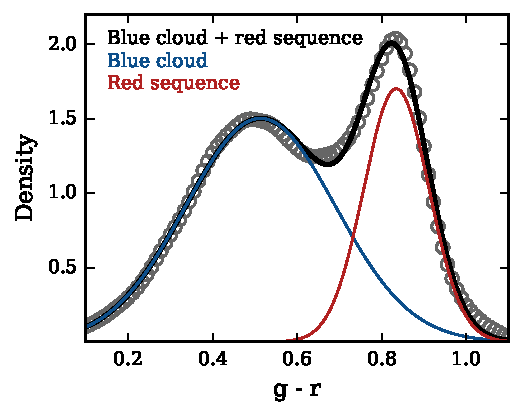
\includegraphics[width=0.8\textwidth]{gr_dist.pdf}
  \caption{$g-r$ colour distributions for low-redshift galaxies in
    SDSS groups.  Circles correspond to the smoothed density
    distribution of the data, the black line shows a double-Gaussian
    fit, and the red and blue lines show the components of the
    double-Gaussian fit corresponding to the red sequence and the blue
  cloud.}
  \label{fig:gr_dist}
\end{figure}

Color is one of the simplest measures with which one can characterize
the properties of a galaxy.  The color of a galaxy is defined as the
difference between the magnitudes of a galaxy in two different bands.
As an example, the $g - r$ colour for a SDSS galaxy would be the
difference between the galaxy's $g$-band magnitude (centred on
$477.0\,\mathrm{nm}$) and $r$-band magnitude (centred on
$623.1\,\mathrm{nm}$).  Many studies have shown the colour
distributions of galaxy populations to be well fit by a
double-Gaussian across many environments \textbf{(REFERENCE)}.  The two
components of the double-Gaussian fit are referred to as the `red
sequence' and the `blue cloud'.  In Fig.~\ref{fig:gr_dist} I show the
$g-r$ colour distribution for a sample of low-redshift ($z < 0.05$)
SDSS group galaxies, and a double-Gaussian fit (black) as well as the
two components corresponding to the blue cloud and the red sequence.
The red sequence peaks at red colours and has a
relatively small dispersion, whereas the blue cloud is a bluer and
broader sub-population.
\par
The overlap region between the red sequence
and the blue cloud is known as the ``green valley'' and is thought to
be a transition region.  It has been hypothesized that galaxies evolve
from the blue cloud, through the green valley, onto the red sequence
over time \textbf{(REFERENCE)}.  An important piece of evidence in
support of
this evolutionary scenario is the Butcher-Oemler (BO) effect.  The BO
effect is an observed positive correlation between the fraction of blue
galaxies within galaxy clusters and redshift, first observed by
\citet{butcher1978} and subsequently observed by many more recent
studies \citep[e.g.][]{butcher1984, ellingson2001, loh2008,
  urquhart2010}.  Therefore it seems that at early times populations
of galaxies in clusters were bluer than they are at present day.    

\subsection{Morphology}

\begin{figure}[!ht]
  \centering
  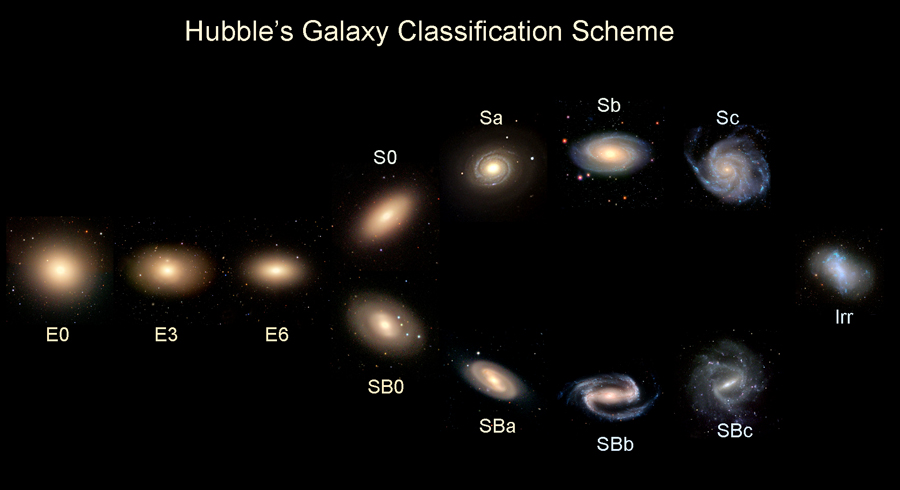
\includegraphics[width=\textwidth]{tuning_fork.jpg}
  \caption{The Hubble tuning fork classification diagram.  Image
    credit: Galaxy Zoo.}
  \label{fig:tuning_fork}
\end{figure}

The first robust classification scheme for galaxies was laid out by
\citet{hubble1926}.  This classification scheme (see
Fig.~\ref{fig:tuning_fork}), which has since become known colloquially
as Hubble's tuning fork diagram, broadly divides the galaxy
population into elliptical and spiral galaxies.  The class of
ellipticals is further sub-divided by ellipticity, $e = 0,1,2,...,7$,
where $e = 10 \times (a-b)/a$, with $a$ and $b$ denoting the major and
minor axis of the ellipse, respectively.  Ellipticals can then be
classified as E$e$, where E$0$ would be perfectly round (in
projection) and E$7$ would be a highly elongated ellipse.  Spiral
galaxies are sub-classified by the brightness of the central region as
well as how tightly coiled are their spiral arms.  Spirals denoted as
S$a$ are galaxies with bright central bulges and tightly wound spiral
arms, galaxies denoted as S$c$ are galaxies with weak bulges and
loosely wound spiral arms, and S$b$ spirals represent an intermediate
class between the two.  Spirals are also divided by the presence of a
bar, or lackthereof, with barred spirals being denoted as SB galaxies.
S$0$ or lenticular galaxies appear to have structure intermediate
between ellipticals and spirals are characterized by a strong bulge
region, as well as the presence of a disc devoid of spiral arms.
Following the nomenclature used by Hubble, it is commonplace to refer
to elliptical and S0 galaxies as ``early-types'' and spiral galaxies
as ``late-types'', due to their positions on the tuning fork diagram.
It is however important to note that this nomenclature refers solely
to the position on the diagram and is agnostic to evolutionary
theories\footnote{Though not always given credit, Hubble was
  very clear on this point stating that the classification was made
  ``without prejudice to theories of evolution'', and that ``temporal
  connotations are made at one's peril''}.
\par
Modern techniques often rely on photometric measurements of 
light profiles of a galaxies to classify morphology.  In particular, two
main measures known as the single \ser index ($n$), and the
bulge-to-total ratio ($B/T$) are commonly used to quantitatively determine
the morphology of a galaxy.
\par
The \ser index, $n$, is a free parameter of the so-called
\ser profile \citep{sersic1968} which often fit to galaxy
intensity profiles.  Using the \ser profile, the intensity of a
galaxy as a function of radius is given by 

\begin{equation}
  I(r) = I_e \exp \{-k [(r/r_e)^{1/n} - 1]\},
\end{equation}

\noindent
where $r_e$ is the effective radius which encloses half of the total
light, $I_e$ is the intensity at the effective radius, and $k$ is a
normalization factor which depends on the S{\'e}rsic index $n$.  In
general, the S{\'e}rsic index runs between $1 \le n \le 8$.  Disc
dominated, spiral galaxies have light profiles which are well fit by a
\ser index of $n \lesssim 2$, with the special case of a purely
exponential disc being given by $n=1$.  Elliptical galaxies have more
centrally concentrated light profiles, and are therefore well fit by
larger \ser indices, $n \gtrsim 2$.  A commonly used empirical law to
describe the brightness profiles of elliptical galaxies is de
Vaucouleurs' law which states that the intensity of an elliptical
galaxies goes as $\log I(r) \propto r^{1/4}$, and this is also just a
special case of the \ser profile with $n=4$.
\par
Instead of modelling the light profile a galaxies as a single
component, bulge + disc decompositions are often used as another
method of classifying the morphology of galaxies.  In this scenario
the light profile of the bulge and disc are modelled separately, it is
common to model the bulge with an $n=4$ de Vaucouleurs profile and the
disc with an $n=1$ exponential profile \citep[e.g.][]{simard2002}, the
sum of these two
components is then the model for the galaxy as a whole.  The fraction
of the total light produced in the bulge component is the bulge-to-total ratio
($B/T$) which is used as a morphological discriminator for galaxies.
Pure elliptical galaxies will have $B/T \to 1$, and pure disc galaxies
will have $B/T \to 0$.  

\subsection{Star formation rates}

\begin{figure}[!ht]
  \centering
  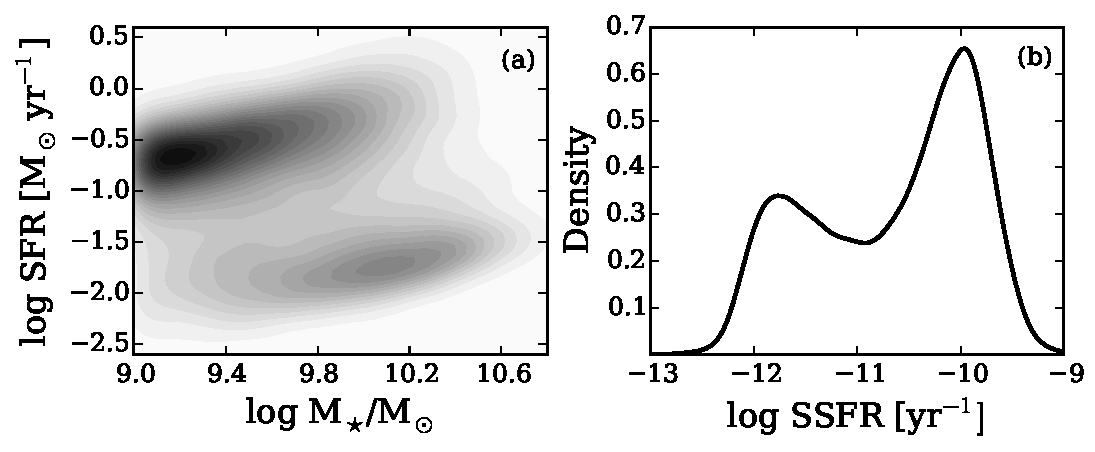
\includegraphics[width=\textwidth]{m_sfr.pdf}
  \caption{Left: Star formation rate versus stellar mass for a sample
    of low-redshift SDSS group galaxies.  Right: Specific star
    formation rate density distribution for a sample of low-redshift
    SDSS group galaxies.}
  \label{fig:m_sfr}
\end{figure}

The star formation rate (SFR) of a galaxy is defined intuitively as the rate
at which a galaxy generates new mass in the form of stars, measured in
units of solar-masses per year ($\Msun\,\mathrm{yr^{-1}}$).  Being
able to accurately determine the SFRs of galaxies is crucial for the
study of galaxy evolution.  Currently there are multiple methods used
to derive SFRs for galaxies, each relying on different aspects of
galactic electromagnetic emission.
\par
One of the most common methods is to derive SFRs from UV or IR
continuum 
emission using conversion factors.  UV continuum emission directly
probes light emitted from young stars and therefore is a strong
indicator of a galaxies SFR.  The largest shortcoming of UV emission
is the fact that the existance of large amounts of interstellar dust
causes galaxies to be relatively opaque to UV photons.  In fact,
approximately half the emission from stars in the Universe is absorbed
and re-emitted by dust in the infrared \citep{kennicutt2012}.
The leads to IR continuum emission from dust being a useful probe of
galaxy SFRs.  As mentioned previously, both UV and IR continuum
luminosities can be converted to SFRs using wavelength-dependent
conversion factors.
\par
In addition to continuum emission, emission line strengths can also be
used as star formation indicators, with the $\mathrm{H}\alpha$ line
being the most commonly used emission line indicator for galaxies in
the local Universe.  As before, using the correct conversion factor
one can determine a SFR estimate from $\mathrm{H}\alpha$ emission, and
similar to the UV continuum, the largest decrement to this method is
dust attenuation.  \citet{kennicutt2012} provide a compilation of up
to date SFR conversion factors for both continuum and line emission,
across a wide range in wavelength.
\par
Another common star formation indicator is the 4000 angstrom break
($\mathrm{D_n}4000$), which refers to the strength of the break at
$4000\,\mathrm{\mathring{A}}$ in a galaxy's spectrum.  Galaxies with
old stellar populations and little recent star formation will show a
strong $\mathrm{D_n}4000$ break due to strong metal absorbtion in the
atmospheres of old stars as well as a lack of UV emission from young,
hot stars \textbf{(REFERENCE)}.  Galaxies with strong recent star
formation will show a correspondingly small break at
$4000\,\mathrm{\mathring{A}}$.
\par
SED fitting...
\par
Across a wide range of environments galaxies
can be divided into two main subpopulations based on their SFRs, those
galaxies which are actively forming stars and those quiescent galaxies
whose star formation has ceased \textbf{(REFERENCE)}.  One way to
define the population of star-forming galaxies is to use the
``star-forming main sequence'' (SFMS).  The SFMS is a tight
correlation between SFR and stellar mass located in the upper region
of $\mathrm{SFR} - M_\star$ plane.  The SFMS for low-redshift galaxies
in SDSS groups is easily visible in Fig.~\ref{fig:m_sfr}(a) ranging
between $\sim -1 < \log \mathrm{SFR} < 0$.  Due to the correlation
between SFR and stellar mass, it is useful to normalize SFR by galaxy
stellar mass, known as the specific star formation rate
($\mathrm{SSFR} = \mathrm{SFR}/M_\star$).  Like the distribution of
galaxy color, the SSFR distribution for galaxy populations is also
bimodal (see Fig.~\ref{fig:m_sfr}(b)).  This bimodality in SSFR
provides another method for distinguishing between star-forming and
passive galaxies.  Recent observations have shown that across
many environments in the local Universe, the division between
the active and quiescent populations (ie.\ the local minimum in the
SSFR distribution) is found at $\log \mathrm{SSFR} \simeq -11$
\citep{wetzel2012}. 

\section{The environmental dependence of galaxy properties}

\subsection{Local density}

One of the first examples of the dependence of galaxy properties on
environment is the observation that the fraction of early-type
galaxies increases with local galaxy number
density\citep{dressler1980}, now known as the Morphology-Density relationship.

% Bibliography
%
\bibliographystyle{apj}
\bibliography{masters-thesis}
